\section{Aufgabe}
\label{sec:chap2:task}

Ziel ist es, eine M"oglichkeit zu schaffen die verschiedenen Enterprise Java Bean Typen mit 
PHP zu implementieren. Hierzu muss zuerst ein Weg gefunden werden der JVM, die den Application Server 
ausf"uhrt die n"otigen Parameter zu "ubergeben die das Laden von Turpitude zur Laufzeit erm"oglichen.
W"unschenswert hierbei w"are, dass die n"otigen Bibliotheken nur einmal beim Start des Application Servers
geladen werden, anstatt jeder installierten Anwendung mitgegeben werden zu m"ussen. Weiterhin muss gew"ahrleistet
werden dass Fehler in der geladenen nativen Bibliothek und in PHP auftretende Fehler m"oglichst nicht zum Absturz des
Application Servers f"uhren, um eine Beeintr"achtigung anderer, im selben Container laufender Applikationen ausschlie\ss en 
zu k"onnen. Ein weiteres Ziel der urspr"unglichen Aufgabenstellung war die Entwicklung eines Buildsystems das dem
Entwickler das unn"otige Schreiben von sogenanntem "'Boilerplate-Code"', Quelltext der f"ur jede
Applikation immer gleich ist, abnimmt. Der PHP-Entwickler, der EJBs schreiben m"ochte, sollte nach M"oglichkeit
keinerlei Java-Quelltext schreiben m"ussen. Leider kann ein solches Buildsystem aufgrund des kleiner
gewordenen Zeitrahmens nicht implementiert werden, allerdings soll bei der Entwicklung darauf geachtet werden,
dass die sp"atere Entwicklung eines solchen Systems m"oglich bleibt.
Abbildung \ref{fig:phpejb} zeigt das Schema eines Aufrufs einer in PHP implementierten Enterprise Java Bean.

\begin{figure}[h]
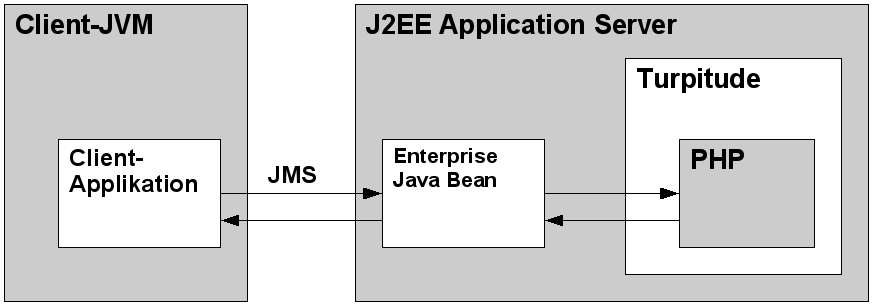
\includegraphics[width=\textwidth]{chap2/img/phpejb.png}
\caption{Aufruf einer PHP-EJB}
\label{fig:phpejb}
\end{figure}

